%%%%%%%%%%%%%%%%%%%%%%%%%%%%%
%%% - Team Organization - %%%
%%%%%%%%%%%%%%%%%%%%%%%%%%%%%
\subsection{Team Organization}
\label{ssec:TeamOrganization}

%Team Organization Chart:
\begin{wrapfigure}[8]{R}{0in}
	\centering
	\raisebox{0pt}[\dimexpr\height-2.5\baselineskip\relax]{
		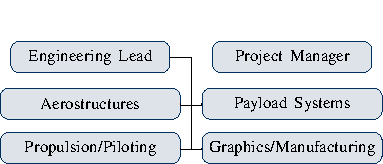
\includegraphics[]{team_organization_chart.pdf}}
	\caption{BYU DBF Team Leadership Organization}
	\label{fig:personnelassignments}
\end{wrapfigure}

%Introduction
\Cref{fig:personnelassignments} depicts the overall organization of our team structure.  Each of the 4 subteams is lead by an individual who answers to the Engineering Lead.  The subteam leads already have the skills described below for their respective subteams, but inexperienced members learn these skills along the way under the mentorship of upperclassmen.




%Team role descriptions continued.

\subsubsection{Engineering Lead} The Engineering Lead has good decision making and leadership skills, qualities the BYU Aeronautics Club seeks to develop in all of its members. 
The Engineering Lead operates as a systems engineer and has a well rounded understanding of the various subsystems and both design and testing experience.
%schedule/milestone chart (since it fits here better.)  Note that you must modify this in the ganttchart.tex file, compile that file, and then compile this file again if you change the schedule.

\subsubsection{Project Manager} The Project Manager acts as a logistical overseer for the team, working with the team leads on the various non-engineering tasks that need to be completed. The Project Manager has excellent organizational and technical writing skills, heading up proposal/report writing, budgeting, and scheduling.
\subsubsection{Aerostructures} The Aerostructures subteam members are responsible for the airframe design and testing. They have expertise in aerodynamic and structural analysis and testing, including design skills in hand calculations and computational analysis tools. They also have experience with wind tunnel, glide, and structural testing methods.
\subsubsection{Propulsion/Piloting} The Propulsion/Piloting subteam focuses on designing and testing the propulsion system efficacy and efficiency. Members also have skills in electronics related to the propulsion system as well as piloting skills used in simulation and flight testing.
\subsubsection{Payload Systems} The Payload Systems subteam is comprised of members with multi-disciplinary skills in structures, manufacture, design, and mechatronics. They bring these skills together to brainstorm, prototype, and test various payload system solutions.
\subsubsection{Graphics/Manufacturing} The Graphics/Manufacturing subteam has skills in CAD design as well as graphical marketing for the team. They also assist in the manufacturing of prototypes and testing apparatus, as well as oversee the construction of the final, full, aircraft.